\subsection{Неравенство треугольника для действительных и комплексных чисел, геометрическое и алгебраическое доказательства.}

\subsubsection*{Неравенство треугольника}
\begin{figure}[h]
    \centering
    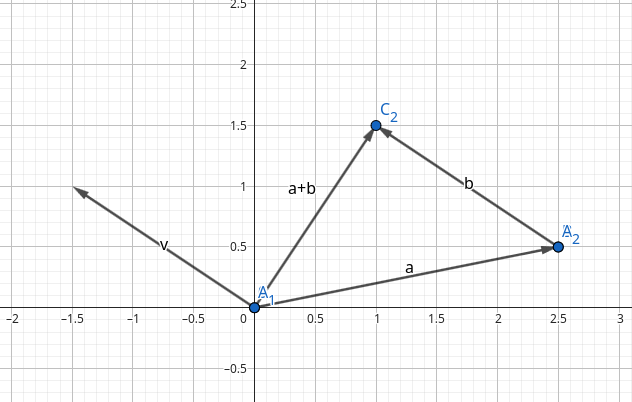
\includegraphics[width=0.5\linewidth]{images/Неравенство(вектора).png}
    \caption{Геометрический смысл неравенства треугольника: длина стороны \( |\vec{a} + \vec{b}| \) не превосходит суммы длин сторон \( |\vec{a}| + |\vec{b}| \).}
    \label{fig:triangle}
\end{figure}
\begin{tcolorbox}
\textbf{Теорема (Неравенство треугольника):}
Для любых комплексных чисел $z_1, z_2$ справедливо:
$$|z_1 + z_2| \leq |z_1| + |z_2|$$
\end{tcolorbox}

\begin{tcolorbox}[title=Доказательство, breakable]
	\[
\begin{aligned}
|z_1 + z_2|^2 &= (z_1 + z_2)(\overline{z_1} + \overline{z_2}) = z_1\overline{z_1} + z_1\overline{z_2} + z_2\overline{z_1} + z_2\overline{z_2} \\
&= |z_1|^2 + z_1\overline{z_2} + \overline{z_1\overline{z_2}} + |z_2|^2 = |z_1|^2 + 2\text{Re}(z_1\overline{z_2}) + |z_2|^2
\end{aligned}
\]
Так как $\text{Re}(w) \le |w|$, то:
\[
\begin{aligned}
|z_1 + z_2|^2 &\le |z_1|^2 + 2|z_1\overline{z_2}| + |z_2|^2 = |z_1|^2 + 2|z_1||z_2| + |z_2|^2 = (|z_1| + |z_2|)^2
\end{aligned}
\]
Извлекая корень, получаем:
$$ |z_1 + z_2| \le |z_1| + |z_2| $$
\end{tcolorbox}

\begin{tcolorbox}[title=Следствие, breakable]
$$||z_1| - |z_2|| \leq |z_1 \pm z_2| \leq |z_1| + |z_2|$$
\end{tcolorbox}
\subsection{Формулы Моргана}
\begin{enumerate}
	\item $A(B+C) = AB + AC$
	\item $A + BC = (A + B)(A + C)$
\end{enumerate}

\begin{tcolorbox}[title=Доказательства]
	\begin{enumerate}
	\item \begin{itemize}
    \item $A(B+C) \subset AB + AC$\\
    $\forall x \in A(B+C) \Rightarrow x \in A \text{ и } x \in B + C$
    \begin{enumerate}
        \item Если $x \in B \Rightarrow$ так как $x \in A$, то $x \in AB \Rightarrow x \in AB + AC$
        \item Если $x \in C \Rightarrow$ так как $x \in A$, то $x \in AC \Rightarrow x \in AB + AC$
    \end{enumerate}
    
    \item $AB + AC \subset A(B+C)$\\
    $\forall x \in AB + AC \Rightarrow x \in AB \text{ или } x \in AC$
    \begin{enumerate}
        \item Если $x \in AB \Rightarrow x \in A \text{ и } x \in B$. Так как $x \in B \Rightarrow x \in B + C$. Итог: $x \in A$ и $x \in B+C \Rightarrow x \in A(B+C)$
        \item Если $x \in AC \Rightarrow x \in A \text{ и } x \in C$. Так как $x \in C \Rightarrow x \in B + C$. Итог: $x \in A$ и $x \in B+C \Rightarrow x \in A(B+C)$
    \end{enumerate}
\end{itemize}
	\item \begin{itemize}
		\item $A + BC \subset (A + B)(A + C)$\\
			$\forall x \in A + BC$
			\begin{enumerate}
				\item Если $x \in A \Rightarrow x \in A + B, x \in A + C \Rightarrow x \in (A + B)(A + C)$
				\item Если $x \in BC \Rightarrow x \in B$ и $x \in C \Rightarrow \forall A\; x \in A + B$ и $x \in A + C \Rightarrow x \in (A + B)(A + C)$
			\end{enumerate}
				\item $(A + B)(A + C) \subset A + BC $\\
					$\forall x \in (A + B)(A + C) \Rightarrow x \in A + B$ и $x \in A + C $
	\begin{enumerate}
		\item $x \in A \Rightarrow x \in A + BC$
		\item $x \not\in A \Rightarrow x \in B$ и $x \in C \Rightarrow x \in BC \Rightarrow \forall A x \in A + BC$
	\end{enumerate}
	\end{itemize}
	\end{enumerate}
\end{tcolorbox}

\subsection{Метод математической индукции (ММИ). Прямая индукция. Формула Бинома Ньютона}

\subsubsection*{Метод математической индукции (ММИ)}
\begin{tcolorbox}
\textbf{Алгоритм доказательства по индукции:}
\begin{enumerate}
    \item \textbf{База индукции:} Проверить утверждение для $n = 1$.
    \item \textbf{Индукционное предположение:} Предположить, что утверждение верно для $n = k$.
    \item \textbf{Индукционный переход:} Доказать, что из этого следует верность утверждения для $n = k+1$ (Прямая индукция).
\end{enumerate}
\end{tcolorbox}

\subsubsection*{Бином Ньютона}
\begin{tcolorbox}
\textbf{Определение.}\\
\textit{Биномиальный коэффициент}:
$C_n^k = \dfrac{n!}{k!(n-k)!}$, где $n,k \in \mathbb{N}_0$\\
\end{tcolorbox}

\begin{tcolorbox}
\textbf{Формула бинома Ньютона:}
$$(a+b)^n = \sum_{k=0}^{n} C_n^k a^{n-k}b^k$$
\end{tcolorbox}

\begin{tcolorbox}[title=Доказательство (ММИ)]
	\begin{enumerate}
		\item \textbf{База индукции ($n=1$):}
		$$ (a+b)^1 = a + b $$
		По формуле:
		$$ \sum_{k=0}^1 C_1^k a^{1-k}b^k = C_1^0 a^1 b^0 + C_1^1 a^0 b^1 = 1\cdot a + 1\cdot b = a+b $$
		Верно.
		
		\item \textbf{Индукционное предположение:}
		Пусть формула верна для $n$:
		$$ (a+b)^n = C_n^0 a^n + C_n^1 a^{n-1}b + \dots + C_n^k a^{n-k}b^k + \dots + C_n^n b^n $$
		
		\item \textbf{Индукционный переход ($n \to n+1$):}
		Рассмотрим $(a+b)^{n+1} = (a+b)(a+b)^n$. Подставим предположение:
		$$ (a+b)^{n+1} = (a+b) \left( C_n^0 a^n + C_n^1 a^{n-1}b + \dots + C_n^n b^n \right) $$
		
		Раскроем скобки, умножив сначала на $a$, а затем на $b$:
		\begin{align*}
			(a+b)^{n+1} &= \mathbf{a} \cdot (C_n^0 a^n + C_n^1 a^{n-1}b + \dots + C_n^n b^n) \\
			            &+ \mathbf{b} \cdot (C_n^0 a^n + C_n^1 a^{n-1}b + \dots + C_n^n b^n)
		\end{align*}
		
		Внесем множители внутрь сумм:
		\begin{align*}
			(a+b)^{n+1} &= \underbrace{C_n^0 a^{n+1} + C_n^1 a^n b + C_n^2 a^{n-1}b^2 + \dots + C_n^n ab^n}_{\text{Умножили на } a} \\
			            &+ \underbrace{C_n^0 a^n b + C_n^1 a^{n-1}b^2 + \dots + C_n^{n-1} ab^n + C_n^n b^{n+1}}_{\text{Умножили на } b}
		\end{align*}
		
		Теперь сгруппируем слагаемые с одинаковыми степенями (подобные члены).
		Заметим, что $a^n b$ есть в обеих строках, $a^{n-1}b^2$ тоже, и т.д.
		
		$$ (a+b)^{n+1} = C_n^0 a^{n+1} + (C_n^1 + C_n^0)a^n b + (C_n^2 + C_n^1)a^{n-1}b^2 + \dots + C_n^n b^{n+1} $$
		
		Воспользуемся свойством биномиальных коэффициентов (правило Паскаля):
		$$ C_n^k + C_n^{k-1} = C_{n+1}^k $$
		
		А также тем, что $C_n^0 = 1 = C_{n+1}^0$ и $C_n^n = 1 = C_{n+1}^{n+1}$.
		Получаем:
		$$ (a+b)^{n+1} = C_{n+1}^0 a^{n+1} + C_{n+1}^1 a^n b + C_{n+1}^2 a^{n-1}b^2 + \dots + C_{n+1}^{n+1} b^{n+1} $$
		
		Что в свернутом виде равно:
		$$ \sum_{k=0}^{n+1} C_{n+1}^k a^{(n+1)-k}b^k $$
		
		Утверждение доказано.
	\end{enumerate}
\end{tcolorbox}


\subsection{ММИ. Обратная индукция. Неравенство между средним арифметическим и средним геометрическим.}

\subsubsection*{Неравенство о средних}
\begin{tcolorbox}
\textbf{Теорема (Неравенство между средним арифметическим и средним геометрическим):}
Для любых $a_1, a_2, \dots, a_n \geq 0$ справедливо:
$$\frac{a_1 + a_2 + \dots + a_n}{n} \geq \sqrt[n]{a_1 a_2 \dots a_n}$$
Равенство достигается тогда и только тогда, когда $a_1 = a_2 = \dots = a_n$.
\end{tcolorbox}

\begin{tcolorbox}[title=Доказательство по ММИ (метод Коши / метод обратой индукции), breakable]
Докажем теорему в три этапа.

\textbf{1. База индукции для степеней двойки ($n=2^m$).}
\begin{itemize}
    \item \textbf{Для $n=2$:} Докажем $\frac{a_1 + a_2}{2} \geq \sqrt{a_1 a_2}$.
    $$(a_1 - a_2)^2 \geq 0 \Rightarrow a_1^2 - 2a_1a_2 + a_2^2 \geq 0 \Rightarrow a_1^2 + 2a_1a_2 + a_2^2 \geq 4a_1a_2 \Rightarrow$$
    $$\Rightarrow (a_1 + a_2)^2 \geq 4a_1a_2 \Rightarrow \frac{a_1 + a_2}{2} \geq \sqrt{a_1 a_2}$$
    \item \textbf{Предположим, неравенство верно для $n = k$.}
    \item \textbf{Докажем для $n = 2k$:}
    $$\frac{a_1 + \dots + a_{2k}}{2k} = \frac{\frac{a_1 + \dots + a_k}{k} + \frac{a_{k+1} + \dots + a_{2k}}{k}}{2} \geq$$
    $$\geq \frac{\sqrt[k]{a_1 \dots a_k} + \sqrt[k]{a_{k+1} \dots a_{2k}}}{2} \geq \sqrt{\sqrt[k]{a_1 \dots a_k} \cdot \sqrt[k]{a_{k+1} \dots a_{2k}}} = \sqrt[2k]{a_1 \dots a_{2k}}$$
\end{itemize}

\textbf{2. Докажем, что если неравенство верно для $n$, то оно верно и для $n-1$.}
Рассмотрим $a_1, a_2, \dots, a_{n-1} \geq 0$. Пусть
$$a_n = \frac{a_1 + a_2 + \dots + a_{n-1}}{n-1}$$
Для набора из $n$ чисел неравенство верно:
$$\frac{a_1 + \dots + a_{n-1} + a_n}{n} \geq \sqrt[n]{a_1 a_2 \dots a_{n-1} a_n}$$
Подставим $a_n$:
$$\frac{(a_1 + \dots + a_{n-1}) + \frac{a_1 + \dots + a_{n-1}}{n-1}}{n} = \frac{a_1 + \dots + a_{n-1}}{n-1} = a_n$$
Таким образом:
$$a_n \geq \sqrt[n]{a_1 a_2 \dots a_{n-1} a_n}$$
Возведём в степень $n$:
$$a_n^n \geq a_1 a_2 \dots a_{n-1} a_n \Rightarrow a_n^{n-1} \geq a_1 a_2 \dots a_{n-1}$$
Извлекая корень $(n-1)$-й степени:
$$a_n \geq \sqrt[n-1]{a_1 a_2 \dots a_{n-1}} \Rightarrow \frac{a_1 + \dots + a_{n-1}}{n-1} \geq \sqrt[n-1]{a_1 a_2 \dots a_{n-1}}$$

\textbf{3. Завершение доказательства.}
Мы доказали, что:
\begin{enumerate}
    \item Неравенство верно для $n=2$ (а значит, для $n=4,8,16,\dots$)
    \item Из верности для $n$ следует верность для $n-1$
\end{enumerate}
Следовательно, неравенство верно для любого натурального $n$.
\end{tcolorbox}
